% Options for packages loaded elsewhere
\PassOptionsToPackage{unicode}{hyperref}
\PassOptionsToPackage{hyphens}{url}
%
\documentclass[
]{article}
\usepackage{amsmath,amssymb}
\usepackage{lmodern}
\usepackage{iftex}
\ifPDFTeX
  \usepackage[T1]{fontenc}
  \usepackage[utf8]{inputenc}
  \usepackage{textcomp} % provide euro and other symbols
\else % if luatex or xetex
  \usepackage{unicode-math}
  \defaultfontfeatures{Scale=MatchLowercase}
  \defaultfontfeatures[\rmfamily]{Ligatures=TeX,Scale=1}
\fi
% Use upquote if available, for straight quotes in verbatim environments
\IfFileExists{upquote.sty}{\usepackage{upquote}}{}
\IfFileExists{microtype.sty}{% use microtype if available
  \usepackage[]{microtype}
  \UseMicrotypeSet[protrusion]{basicmath} % disable protrusion for tt fonts
}{}
\makeatletter
\@ifundefined{KOMAClassName}{% if non-KOMA class
  \IfFileExists{parskip.sty}{%
    \usepackage{parskip}
  }{% else
    \setlength{\parindent}{0pt}
    \setlength{\parskip}{6pt plus 2pt minus 1pt}}
}{% if KOMA class
  \KOMAoptions{parskip=half}}
\makeatother
\usepackage{xcolor}
\usepackage[margin=1in]{geometry}
\usepackage{longtable,booktabs,array}
\usepackage{calc} % for calculating minipage widths
% Correct order of tables after \paragraph or \subparagraph
\usepackage{etoolbox}
\makeatletter
\patchcmd\longtable{\par}{\if@noskipsec\mbox{}\fi\par}{}{}
\makeatother
% Allow footnotes in longtable head/foot
\IfFileExists{footnotehyper.sty}{\usepackage{footnotehyper}}{\usepackage{footnote}}
\makesavenoteenv{longtable}
\usepackage{graphicx}
\makeatletter
\def\maxwidth{\ifdim\Gin@nat@width>\linewidth\linewidth\else\Gin@nat@width\fi}
\def\maxheight{\ifdim\Gin@nat@height>\textheight\textheight\else\Gin@nat@height\fi}
\makeatother
% Scale images if necessary, so that they will not overflow the page
% margins by default, and it is still possible to overwrite the defaults
% using explicit options in \includegraphics[width, height, ...]{}
\setkeys{Gin}{width=\maxwidth,height=\maxheight,keepaspectratio}
% Set default figure placement to htbp
\makeatletter
\def\fps@figure{htbp}
\makeatother
\setlength{\emergencystretch}{3em} % prevent overfull lines
\providecommand{\tightlist}{%
  \setlength{\itemsep}{0pt}\setlength{\parskip}{0pt}}
\setcounter{secnumdepth}{-\maxdimen} % remove section numbering
\ifLuaTeX
  \usepackage{selnolig}  % disable illegal ligatures
\fi
\IfFileExists{bookmark.sty}{\usepackage{bookmark}}{\usepackage{hyperref}}
\IfFileExists{xurl.sty}{\usepackage{xurl}}{} % add URL line breaks if available
\urlstyle{same} % disable monospaced font for URLs
\hypersetup{
  pdftitle={Prediction of Readmission for Diabetic Patients},
  pdfauthor={Anran Yao, Mingrui Li, Wenjing Li},
  hidelinks,
  pdfcreator={LaTeX via pandoc}}

\title{Prediction of Readmission for Diabetic Patients}
\author{Anran Yao, Mingrui Li, Wenjing Li}
\date{December 16, 2022}

\begin{document}
\maketitle

\hypertarget{introduction}{%
\subsection{1.Introduction}\label{introduction}}

Diabetes is a chronic disease that affects millions of people around the
world with more than one tenths of Americans suffering from it. Managing
diabetes can be a complex and challenging task as the overall
readmission rate among diabetic patients is 18.9\% \(^{[1]}\), which is
much higher than the readmission rate for other patients (8.5--13.5\%)
\(^{[2]}\). One important aspect of diabetes management is the
prevention of hospital readmission, as frequent readmission can be
costly and may negatively impact patient\(^{[3]}\) outcomes. In this
study, we aimed to develop a prediction model for readmission rates for
diabetic patients using a dataset from Kaggle. Prediction methods
including logistic regression, naive bayesian, decision tree and random
forest were used, and their performances were evaluated by AUC, ROC, and
confusion matrix.

\hypertarget{methods}{%
\subsection{2.Methods}\label{methods}}

\textbf{2.1 Study Population }\\
The dataset we used in this study was provided by Kaggle which contained
information on diabetic patients who were hospitalized. The data range
from 1999 to 2008 included a total of 101,766 samples and 50 variables,
with each sample representing an unique observation of admission. The
dataset included demographic and physical features of patients,
medications, number of certain medical record and diagnoses.

\textbf{2.2 Data cleaning}\\
Before analysis, the dataset was cleaned and preprocessed to remove any
missing or irrelevant data. Variables with more than 40\% missingness
were excluded such as weight, payer code and medical specialty.
Variables that are not representative such as IDs were also excluded. We
also removed variables of medications that are rarely used in patients
because of their limited application to the general diabetic population.
Rows containing missing values after selecting variables were directly
deleted. After exclusion, there were 99492 observations with 30
variables.

\textbf{2.3 Variables}\\
The outcome of this study is a categorical variable that indicates days
to inpatient readmission. The outcome has 3 values, ``\textless30'' or
``\textgreater30'' if the patient was readmitted in less or more than 30
days and ``No'' for no record of readmission. We convert the outcome to
binary by considering ``No'' as 0, readmitted as 1 no matter less or
more than 30 days. The variables diagnose 1, diagnose 2 and diagnose 3
were merged to find the 6 most frequent ICD-9 codes among diabatic
patients and considered them as a new variable. Those codes with decimal
points belong to the same diagnosis category to its rounded value, for
instance 250.01 and 250 both indicate diabate.The following variables
were concluded in this study: number\_inpatient, which reflects the
number of inpatient visits of the patient in the year preceding the
encounter; number\_enmergency, which represents the number of emergency
visits; num\_medications, which indicates the number of distinct generic
names administered during the encounter; diabetesMed, to demonstrate if
there was any diabetic medication prescribed; age, which grouped in
10-year intervals.

\textbf{2.4 Descriptive analysis}\\
Inpatient Outpatient Emergency Age diabetesMed

\hypertarget{methodology}{%
\subsection{3. Methodology}\label{methodology}}

To predict readmission rates, we splitted the data into training(70\%)
and testing(30\%), and used four different prediction methods to train
the dataset, including logistic regression, naive bayesian, decision
tree and random forest.

\textbf{3.1 Logistic Regression}\\
Logistic regression is a statistical method that is used to predict a
binary outcome, such as whether a patient will be readmitted or not in
this study. It is based on the principle of linear regression, which
means that it makes predictions based on a linear combination of the
input features. The readmission is transformed into a binary outcome
using a logistic function.

\textbf{3.2 Naive Bayesia}\\
Naive Bayesian is a probabilistic machine learning method that is based
on the principle of Bayesian probability. It is called ``naive'' because
it assumes that all of the features in the dataset are independent of
one another, which is not always the case in real-world data. Despite
this assumption, naive Bayesian algorithms can still be very effective
at making predictions in many situations.

\textbf{3.3 Decision Tree}\\
Decision tree is a machine learning algorithm that is used to make
predictions based on a tree-like model of decisions. It works by
dividing the input data into smaller and smaller subsets based on the
values of the input features. At each step, the algorithm chooses the
feature that provides the most information about the target variable,
and splits the data accordingly. The resulting tree can then be used to
make predictions by following the path through the tree that leads to
the most likely outcome. In order to allow the tree to fully grow and to
prune its branches afterwards, we tuned the parameters of the decision
tree by grid search during the model prediction process, and used the
tuned parameters to predict the readmission outcome of test data.

\textbf{3.4 Random Forest}\\
Random forest is an ensemble learning method that is used to make
predictions based on the collective input of a group of decision trees.
It works by creating a large number of decision trees using random
subsets of the input data, and then averaging the predictions made by
each tree. After plotting different numbers of trees to the error, we
decided to use 100 trees in the prediction. By grid search of the
parameters, mtry(number of variables randomly sampled as candidates at
each split) was set to 4.

\textbf{3.5 Model Comparison Methods}\\
To evaluate the performance of the prediction models, we used three
evaluation metrics: AUC, ROC, and confusion matrix. AUC (area under the
curve) is a measure of the performance of a binary classification model,
with a value of 1 indicating perfect performance and a value of 0.5
indicating random performance. ROC (receiver operating characteristic)
is a plot of the true positive rate against the false positive rate, and
is used to evaluate the performance of a binary classification model.
Confusion matrix is a table that shows the number of true positive, true
negative, false positive, and false negative predictions made by a
classification model.

\hypertarget{results}{%
\subsection{4.Results}\label{results}}

\textbf{4.1 Model Comparison}\\

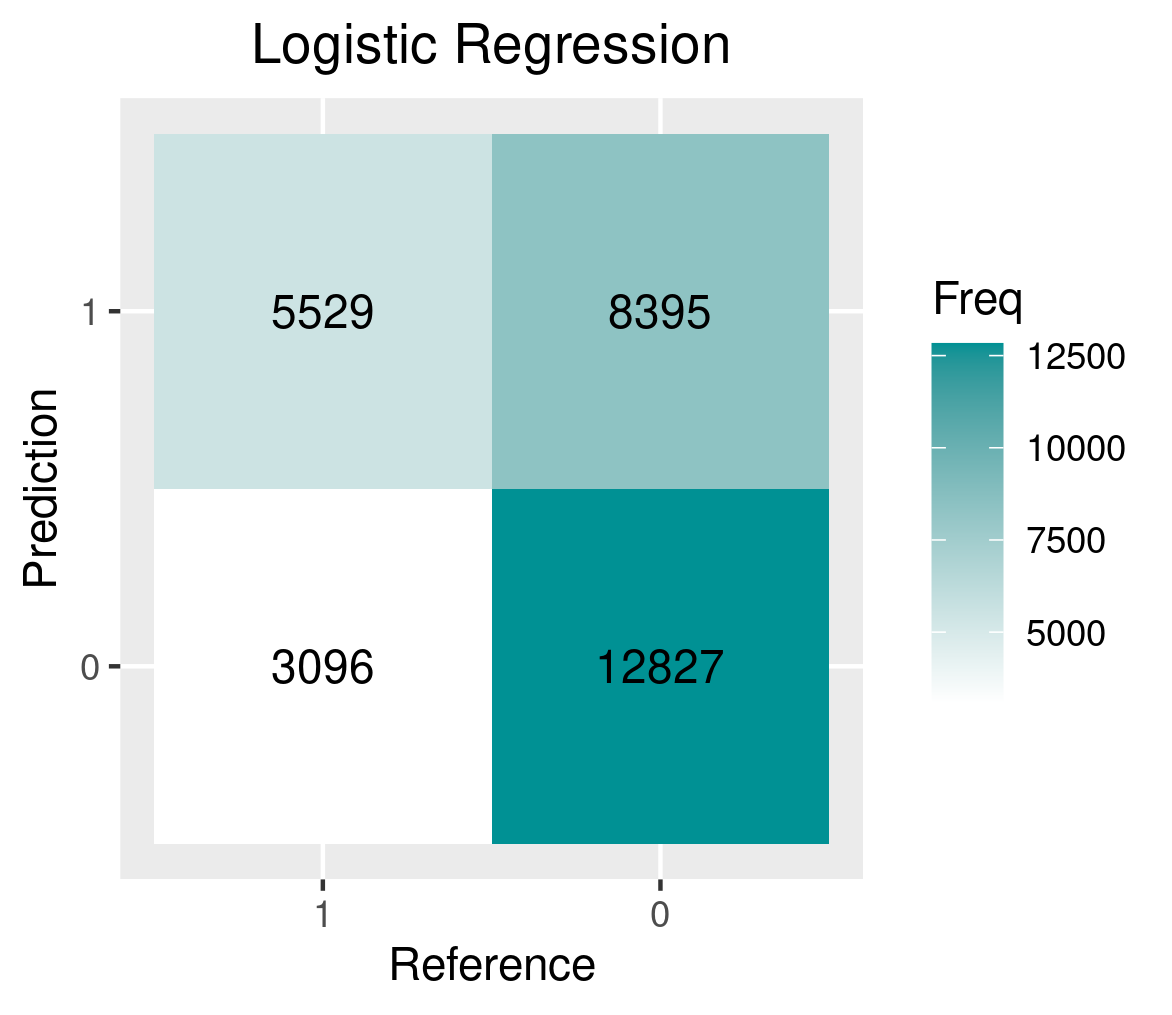
\includegraphics[width=0.4\textwidth,height=\textheight]{pltcm_gg_glm.png}
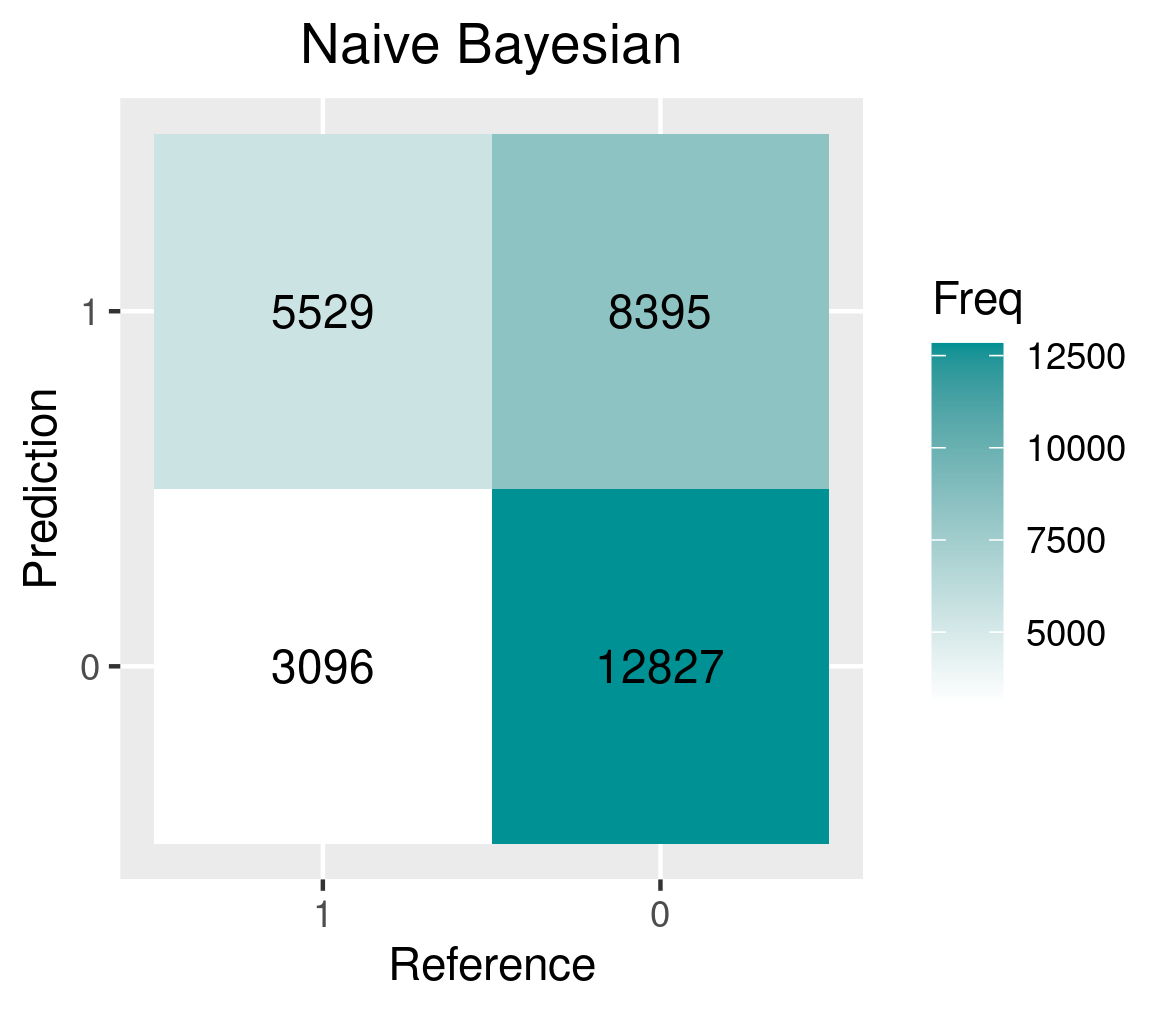
\includegraphics[width=0.4\textwidth,height=\textheight]{pltcm_gg_nb.png}

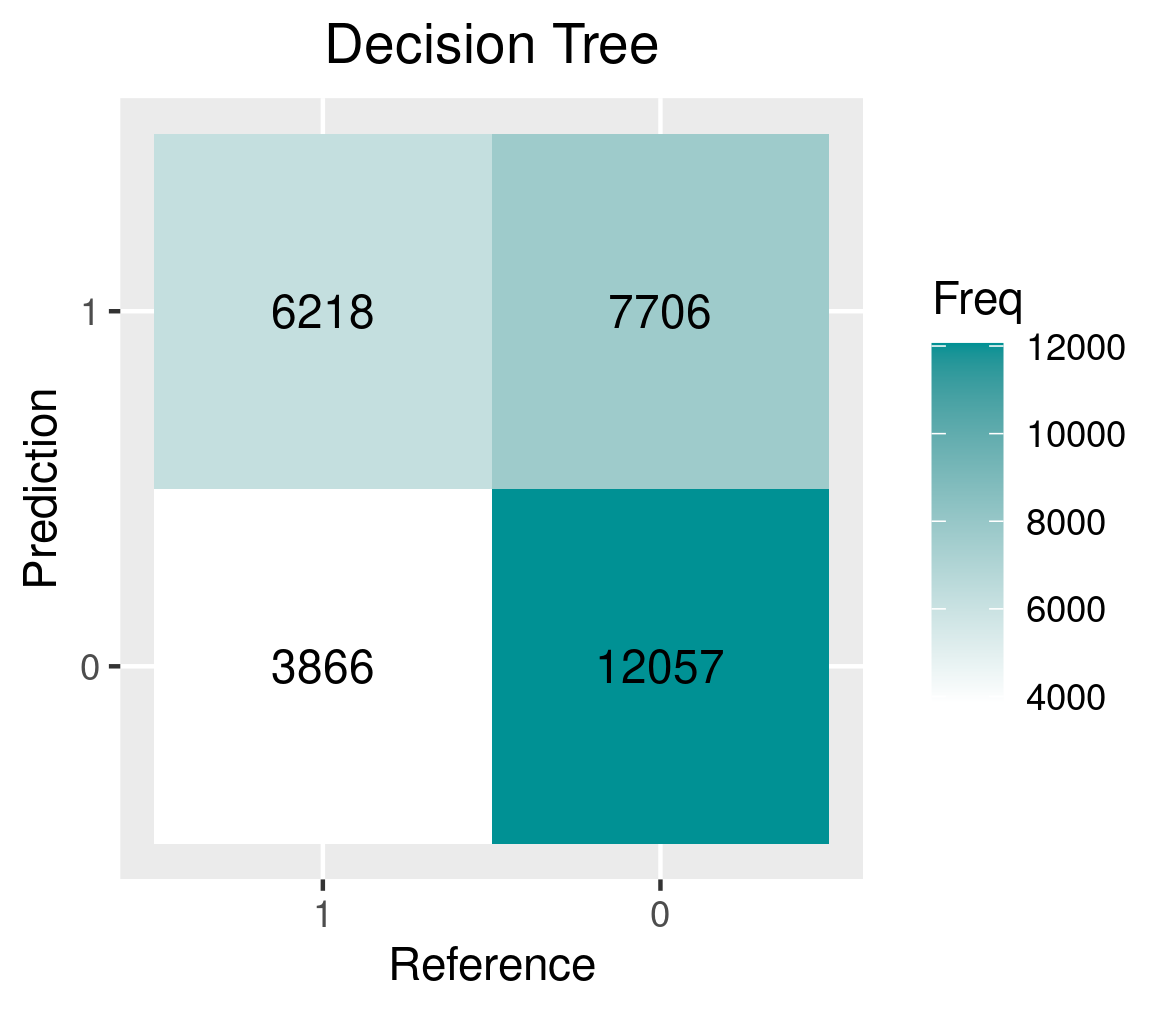
\includegraphics[width=0.4\textwidth,height=\textheight]{pltcm_gg_rp.png}
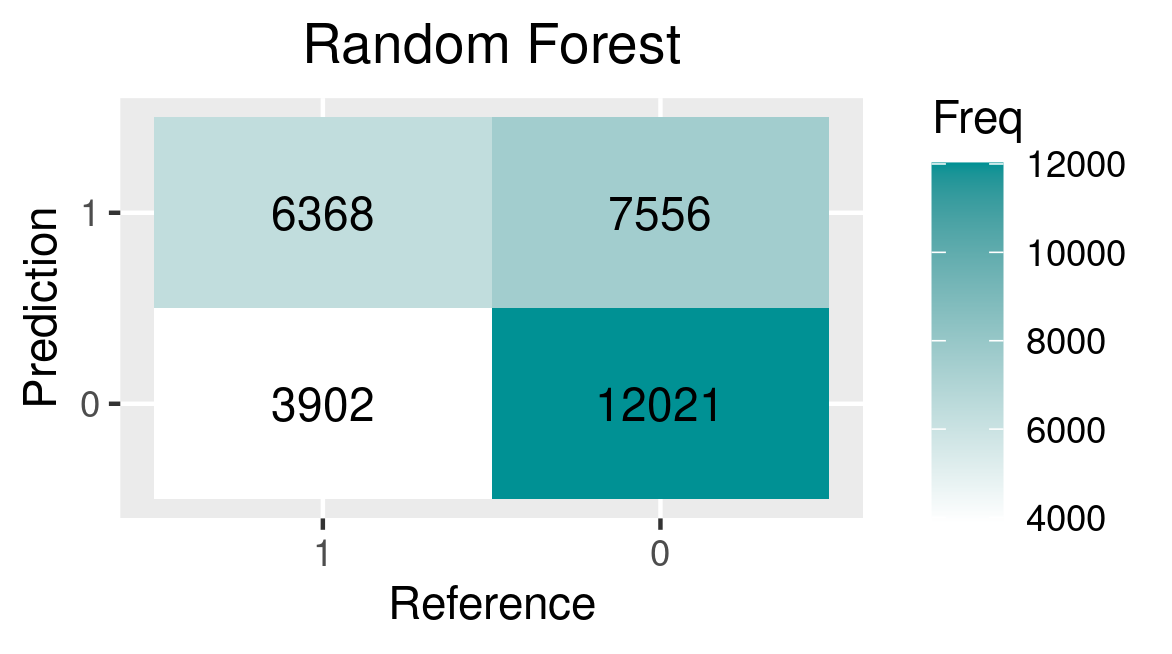
\includegraphics[width=0.4\textwidth,height=\textheight]{pltcm_gg_rf.png}

Figure 1: Confusion Matrices of Prediction

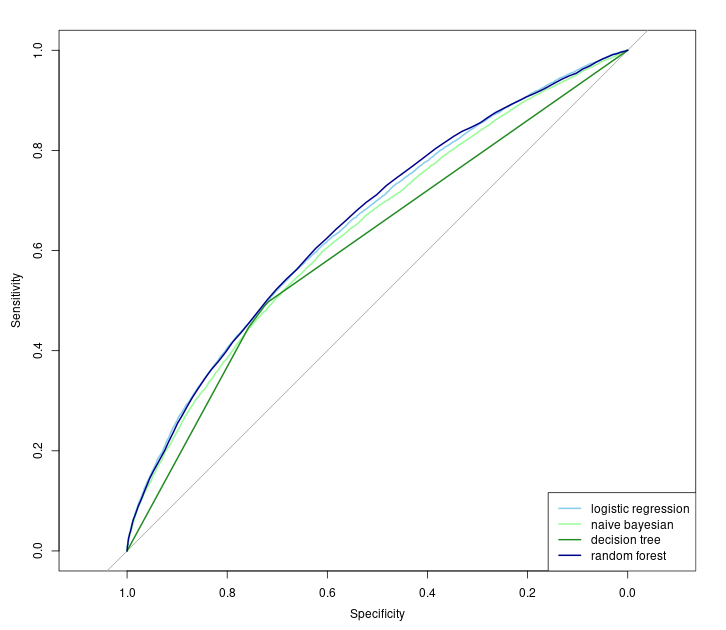
\includegraphics[width=0.5\textwidth,height=\textheight]{ROC.png}     
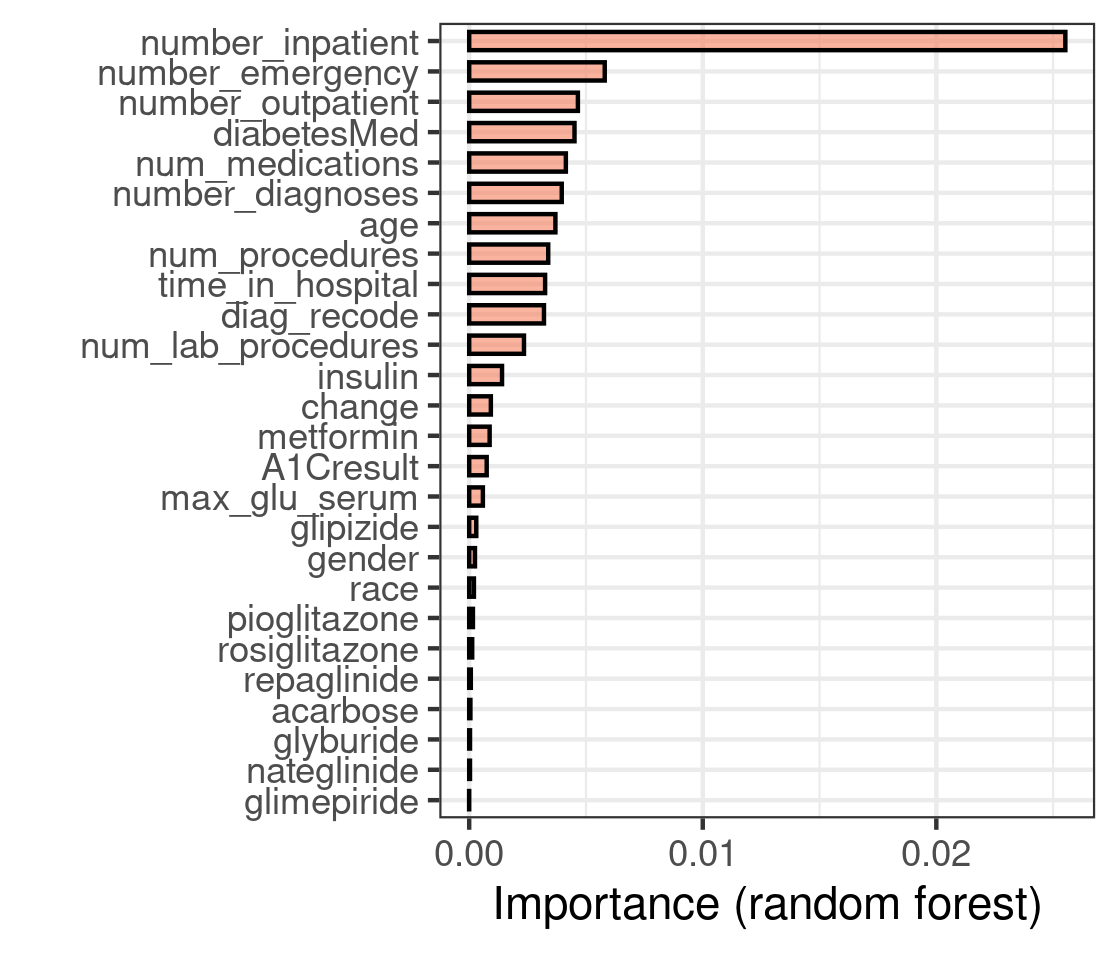
\includegraphics[width=0.5\textwidth,height=\textheight]{Importance_rf.png}

Figure 2: ROC Plot Figure 3: Importance of Variables

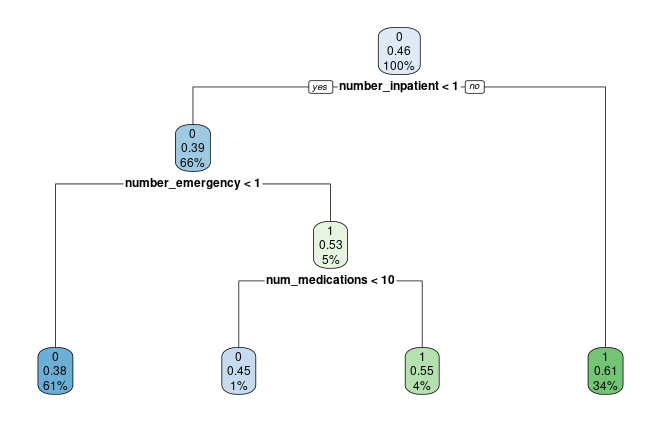
\includegraphics[width=0.8\textwidth,height=\textheight]{tuned_decisiontree.png}

Figure 4: Result of Decision Tree

\begin{longtable}[]{@{}lrrrr@{}}
\caption{Confusion Matrix Parameters and Area Under
Curve}\tabularnewline
\toprule()
& Logistic Regression & Naive Bayesian & Decision Tree & Random
Forest \\
\midrule()
\endfirsthead
\toprule()
& Logistic Regression & Naive Bayesian & Decision Tree & Random
Forest \\
\midrule()
\endhead
Accuracy & 0.615 & 0.587 & 0.612 & 0.616 \\
Specificity & 0.806 & 0.913 & 0.757 & 0.755 \\
Sensitivity & 0.397 & 0.214 & 0.447 & 0.457 \\
PosPredValue & 0.641 & 0.682 & 0.617 & 0.620 \\
NegPredValue & 0.604 & 0.570 & 0.610 & 0.614 \\
AUC & 0.654 & 0.641 & 0.610 & 0.656 \\
\bottomrule()
\end{longtable}

After conducting the prediction methods to train data and testing the
model performance, we get the confusion matrices of the models. Random
Forest performed the best in the testing data with an accuracy of
61.6\%, while Naive Bayesian got the lowest accuracy of 58.7\%. The
sensitivity of each model is relatively poor, being below 50\%, which
means that the rate of missing diagnoses is high. Naive Bayesian got the
highest specificity (91.3\%), followed by logistic regression (80.6\%),
showing that our prediction model can recognize as many negative cases
as possible, without misjudgment of readmission. Area Under Curve and
ROC Plot (Figure 2) got the same result in accuracy, indicating that
Random Forest got the best performance, and logistic regression was the
second.

The importance of variables given by random forest prediction model is
given by Figure 3. Number of inpatient visits provided the highest
contribution rate, followed by the numbers of emergency and outpatient
visits, indicating that the numbers of visits are the most important
predictors of readmission. Comparing the decision tree results (Figure
4), we can see that the number of inpatient visits has the greatest gain
in information about whether or not to be readmitted in the future,
i.e., the highest purity. The decision tree selects the number of
medications administered during the encounter in the third branch,
indicating that this variable has a strong effect on the model. However,
Random Forest combines multiple decision trees, which can help to reduce
the overall variance of the predictions, which explains why the random
forest has the best predictive performance on our study.

Ihe importance of variables given by random forest prediction model is
given by Figure 3. Number of inpatient visits provided the highest
contribution rate, followed by the numbers of emergency and outpatient
visits, indicating that the numbers of visits are the most important
predictors of readmission. Comparing the decision tree results (Figure
4), we can see that the number of inpatient visits has the greatest gain
in information about whether or not to be readmitted in the future,
i.e., the highest purity. The decision tree selects the number of
medications administered during the encounter in the third branch,
indicating that this variable has a strong effect on the model. However,
Random Forest combines multiple decision trees, which can help to reduce
the overall variance of the predictions, which explains why the random
forest has the best predictive performance on our study.

\textbf{4.2 Prediction Example}\\
When a patient is discharged from the hospital, we can calculate the
probability of readmission based on their registration information to
facilitate future follow-up arrangements. Here is a prediction example
of our model. Let's say a patient aged between 30 to 40, stayed in
hospital for 2 days during the encounter, had 44 lab tests, and took 16
distinct of medications, no outpatient/emergency/inpatient visit, got 7
diagnoses, main diagnose was diabetes and took insulin, did not do blood
glucose tests in the year preceding the encounter. According to the
random forest model, the patient's probability of readmission is 30.0\%,
while logistic gives 37.4\%, naive bayesian gives 13.8\%, and decision
tree gives 30.\%. From model comparison results, we can use the result
of random forest as the final prediction of readmission.

\hypertarget{conclusion-and-discussion}{%
\subsection{5.Conclusion and
Discussion}\label{conclusion-and-discussion}}

The performance of models is not ideal. The first reason may be the
quality of the data. This dataset is from 1999 to 2008 which may be hard
to collect a complete dataset at that period. Glucose level is that may
lack crucial test results such as glucose level. Second, other model
improvement methods such as cross validation may increase the robustness
of the model, which we may consider in the future.

\hypertarget{references}{%
\subsubsection{References}\label{references}}

{[}1{]} Judy Y. Chen, M.D., M.S.H.S., Qiufei Ma, Ph.D., Hua Chen, M.D.,
and Irina Yermilov, M.D., M.P.H.T.M. \emph{New Bundled World: Quality of
Care and Readmission in Diabetes Patients.}
\url{https://www.pharllc.com/wp-content/uploads/2019/12/Chen-J-Diabetes-Sci-Technol-2012.pdf}
{[}2{]} Ostling, S., Wyckoff, J., Ciarkowski, S.L. et al.~\emph{The
relationship between diabetes mellitus and 30-day readmission rates.}
\url{https://clindiabetesendo.biomedcentral.com/articles/10.1186/s40842-016-0040-x\#citeas}
{[}3{]} Rubin, D. J. (2015). Hospital readmission of patients with
diabetes. \emph{Current diabetes reports}, 15(4), 1-9.

\end{document}
